% !TeX spellcheck = de_DE
% !TeX root = kristallographie_skript.tex
\begin{sheet}

\begin{problem}
Andrea und ich haben Polyeder mitgebracht. Bestimme
\begin{subproblem}
Die Anzahl der Symmetrien, aufgeschlüsselt nach Typen (Spiegelungen, 2-, 3-, 4-zählige Drehungen, ...)
\end{subproblem}
\begin{subproblem}
Welche Polyeder gleich viele Symmetrien haben
\end{subproblem}
\begin{subproblem}
Welche Polyeder \enquote{die gleiche} Symmetriegruppe haben (ohne jetzt genau zu sagen, was das heißt. Wir präzisieren das später.)
\end{subproblem}
für so viele Polyeder, wie du Lust hast.
\end{problem}

\begin{problem}
Sei $G$ eine Gruppe und $g\in G$ ein Element dieser Gruppe.

Zeige zunächst, dass die folgenden Abbildungen $G\to G$ bijektiv sind:
\begin{subproblem}
\enquote{Linksmultiplikation}: $\lambda_g(x):=gx$.
\end{subproblem}
\begin{subproblem}
\enquote{Rechtsmultiplikation}: $\rho_g(x):=xg$.
\end{subproblem}
\begin{subproblem}
\enquote{Konjugation}: $\kappa_g(x):=gxg^{-1}$.
\end{subproblem}
In anderen Worten: Die Gleichungen $gx=y$, $xg=y$ bzw. $gxg^{-1} = y$ sind für alle $y\in G$ eindeutig nach $x$ lösbar.

\begin{subproblem}[difficulty={mittel}]
Umgekehrt: Es sei umgekehrt $X$ eine nichtleere Menge und $\ast: X\times X\to X$ eine assoziative Verknüpfung, die folgende Eigenschaft hat:
\[\forall g,y\in X: (\exists! x\in X: g \ast x=y) \wedge (\exists! x\in X: x \ast g=y)\]
d.h. die Gleichungen $g \ast x=y$ und $x \ast g=y$ sind eindeutig nach $x$ lösbar, egal, was $g$ und $y$ sind. Zeige, dass $(X,\ast)$ eine Gruppe ist.
\end{subproblem}
\end{problem}

\begin{problem}
Mit den Bezeichnungen der vorherigen Aufgabe beweise, dass ferner folgende Aussagen gelten für alle $g,h\in G$:
\begin{subproblem}
$\lambda_g \circ \rho_h = \rho_h \circ \lambda_g$.
\end{subproblem}
\begin{subproblem}
$\lambda_g \circ \lambda_h = \lambda_{gh}$ und $\rho_g \circ \rho_h = \rho_{gh}$.
\end{subproblem}
\begin{subproblem}
$\kappa_g\circ\kappa_h = \kappa_{gh}$.
\end{subproblem}
\begin{subproblem}
Die Konjugation $\kappa_g$ ist ein Homomorphismus:

$\forall x,y\in G: \kappa_g(xy) = \kappa_g(x)\kappa_g(y)$.
\end{subproblem}
(Man mache sich klar, dass die Gleichungen in a. und in b. exakt äquivalent zum Assoziativgesetz sind!)
\end{problem}



\begin{problem}[title={Diedergruppen / Symmetrien des regulären $n$-Ecks}]
Es seien $\rho_0,\rho_{2\pi/3},\rho_{4\pi/3}, \sigma_0, \sigma_{\pi/3}, \sigma_{2\pi/3}$ die Abbildungen in \ref{figure:Dih_6}.
\begin{figure}[ht]

\begin{tabular}{c|c|c}
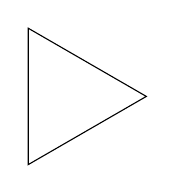
\begin{tikzpicture}
\draw (0:1cm) -- (120:1cm) -- (240:1cm) -- cycle;
\end{tikzpicture}
&
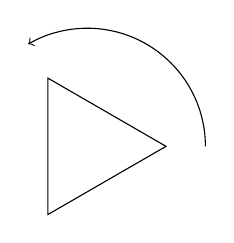
\begin{tikzpicture}
\draw (0:1cm) -- (120:1cm) -- (240:1cm) -- cycle;

\draw[->] (0:1.5cm) arc[radius=1.5cm, start angle=0,end angle=120];
\end{tikzpicture}
&
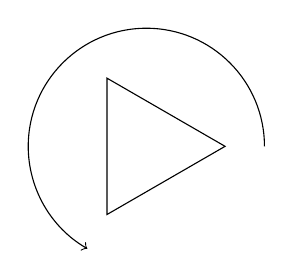
\begin{tikzpicture}
\draw (0:1cm) -- (120:1cm) -- (240:1cm) -- cycle;

\draw[->] (0:1.5cm) arc[radius=1.5cm, start angle=0,end angle=240];
\end{tikzpicture}
\\ \hline
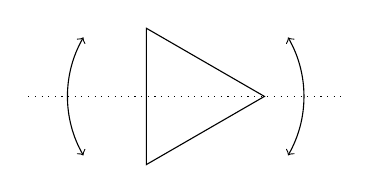
\begin{tikzpicture}
\draw (0:1cm) -- (120:1cm) -- (240:1cm) -- cycle;

\draw[dotted] (180:2cm) -- (0:2cm);

\draw[<->] (150:1.5cm) arc[radius=1.5cm, start angle=150,end angle=210];
\draw[<->] (-30:1.5cm) arc[radius=1.5cm, start angle=-30,end angle=30];
\end{tikzpicture}
&
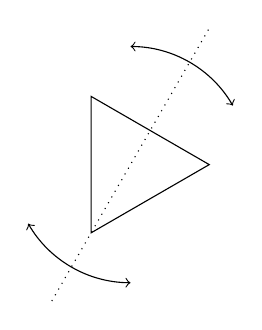
\begin{tikzpicture}
\draw (0:1cm) -- (120:1cm) -- (240:1cm) -- cycle;

\draw[dotted] (240:2cm) -- (60:2cm);

\draw[<->] (30:1.5cm) arc[radius=1.5cm, start angle=30,end angle=90];
\draw[<->] (210:1.5cm) arc[radius=1.5cm, start angle=210,end angle=270];
\end{tikzpicture}
&
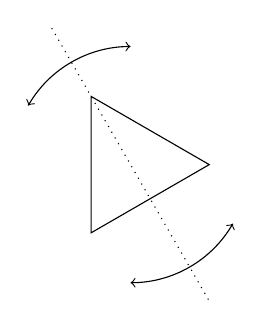
\begin{tikzpicture}
\draw (0:1cm) -- (120:1cm) -- (240:1cm) -- cycle;

\draw[dotted] (120:2cm) -- (300:2cm);

\draw[<->] (90:1.5cm) arc[radius=1.5cm, start angle=90,end angle=150];
\draw[<->] (-30:1.5cm) arc[radius=1.5cm, start angle=-30,end angle=-90];
\end{tikzpicture}
\end{tabular}
\caption{Die sechs Elemente von $Aut(\triangleright)$; Obere Zeile von links nach rechts: $\rho_0,\rho_{2\pi/3},\rho_{4\pi/3}$, untere Zeile: $\sigma_0,\sigma_{\pi/3}, \sigma_{2\pi/3}$.}
\label{figure:Dih_6}
\end{figure}
Überlege dir geometrisch, dass ...
\begin{enumerate}
\item ... $(\Set{\rho_0,\rho_{\pi/3},\rho_{2\pi/3},\sigma_0,\sigma_{\pi/3}, \sigma_{2\pi/3}},\circ)$ eine Gruppe ist.
\item ... diese Gruppe nicht abelsch ist.
\item $\sigma_\theta\circ \rho_\alpha\circ\sigma_\theta^{-1} = \rho_{-\alpha}$ für alle $\alpha$ und $\theta$.
\end{enumerate}
Bonus: Beschreibe eine analoge Gruppe für das regelmäßige $n$-Eck. Wie viele Elemente hat diese?

Allgemein: Ist $\rho_\alpha$ die Rotation um $\alpha\in\IR$ und $\sigma_\theta$ die Spiegelung an der Achse, die um $\theta\in\IR$ gegen die $x$-Achse geneigt ist, dann gilt 
\[\rho_\alpha \circ \rho_{\alpha'} = \rho_{\alpha+\alpha'},\quad \rho_\alpha \circ \sigma_\theta = \sigma_{\alpha/2 + \theta},\quad \sigma_\alpha\circ\rho_\alpha = \sigma_{\theta - \alpha/2} \;\text{und}\; \sigma_{\theta}\circ\sigma_{\theta'} = \rho_{2(\theta-\theta')}\]
für alle $\alpha,\alpha'\in\IR$, $\theta,\theta'\in\IR$.

Dann 
\[Dih(n):=\Aut(n\text{-Eck}) = \Set{\rho_{k\frac{2\pi}{n}}, \sigma_{l\frac{\pi}{n}} | 0\leq k,l<n}\]
für alle $n\geq 3$.
\end{problem}

\begin{problem}[title={Automorphismen des affinen Raums}]
\begin{subproblem}
Zeige, dass die Menge
\[Aff(\IR):=\Set{f:\IR\to\IR | \exists a\in\IR\setminus\Set{0} \exists b\in\IR \forall x\in\IR: f(x)=ax+b}\]
mit der Komposition als Verknüpfung eine Gruppe bildet.
\end{subproblem}
\begin{subproblem}
Allgemeiner: Zeige, dass
\[Aff(\IR^n):=\Set{f:\IR^n\to\IR^n | \exists A\in GL_n(\IR), b\in\IR^n: \forall x\in\IR^n: f(x)=Ax+b}\]
mit der Komposition eine Gruppe bildet.
\end{subproblem}
Dies ist die sogenannte \udot{affine Gruppe}.

\begin{subproblem}
Beweise, dass $\Isom(\IR^n)\leq Aff(\IR^n)$ ist.
\end{subproblem}
\end{problem}

\begin{problem}[title={Möbius-Transformationen / Automorphismen der projektiven Geraden}]
Zeige, dass die Menge der formalen Ausdrücke (im Gegensatz zu \enquote{Funktionen}, d.h. wir ignorieren Probleme mit Definitionsbereichen) der Form $\frac{aZ+b}{cZ+d}$ mit einer Unbekannten $Z$ und komplexen Zahlen $a,b,c,d\in\IC$ mit $ad-bc\neq 0$ eine Gruppe bzgl. der Verknüpfung \enquote{in einander einsetzen} bildet, d.h.
\[\frac{aZ+b}{cZ+d} \circ \frac{a'Z+b'}{c'Z+d'} := \frac{a\frac{a'Z+b'}{c'Z+d'}+b}{c\frac{a'Z+b'}{c'Z+d'}+d}\]

(Hinweis: Wenn man den Bruch vereinfacht, kommen Koeffizienten heraus, die etwas mit $2\times 2$-Matrizen zu tun haben. Wir finden so die Gruppe $PGL_2(\IC)$.)
\end{problem}



\begin{problem}
Wir schreiben eine Permutation $\pi\in Sym(n)$ auch wie folgt als zweizeilige Wertetabelle auf:
\[\pi = \begin{pmatrix} 1& 2 & \cdots & n \\ \pi(1) & \pi(2) & \cdots & \pi(n)\end{pmatrix}\]

Berechne die folgenden Produkte in $Sym(6)$:
\begin{enumerate}
\item $\begin{pmatrix} 1 & 2 & 3 & 4 & 5 & 6 \\ 3 & 5 & 1 & 2 & 4 & 6\end{pmatrix} \circ \begin{pmatrix} 1 & 2 & 3 & 4 & 5 & 6 \\ 1 & 4 & 3 & 6 & 5 & 2\end{pmatrix}$
\item $\begin{pmatrix} 1 & 2 & 3 & 4 & 5 & 6 \\ 4 & 3 & 6 & 2 & 5 & 1\end{pmatrix} \circ \begin{pmatrix} 1 & 2 & 3 & 4 & 5 & 6 \\ 6 & 5 & 4 & 3 & 2 & 1\end{pmatrix}$
\end{enumerate}
\end{problem}

\begin{problem}[title={Zyklenzerlegung}]
Seien $n,r\in\IN$ und $a_1,\ldots,a_r\in\set{1,\ldots,n}$.

Der \udot{$r$-Zyklus} $(a_1 a_2 \ldots a_r)$ ist diejenige Permutation $\sigma\in Sym(n)$, die $a_1\mapsto a_2, a_2\mapsto a_3, \ldots, a_{r-1}\mapsto a_r, a_r\mapsto a_1$ und $x\mapsto x$ für alle anderen Elemente erfüllt.

\begin{subproblem}[difficulty={leicht}]
Schreibe die Permutation $\begin{pmatrix} 1 & 2 & 3 \\ 2 & 3 & 1 \end{pmatrix}$ als Produkt von zwei Transpositionen (:= 2-Zyklen).
\end{subproblem}

Zwei Zyklen heißen \udot{disjunkt}, wenn die Mengen der jeweils bewegten Elemente disjunkt sind. $(123)$ und $(45)$ sind disjunkt, $(123)$ und $(315)$ nicht.
\begin{subproblem}[difficulty={leicht bis mittel}]
Beweise: \emph{Jede} Permutation ist ein Produkt von disjunkten Zyklen.

(Hinweis: Zeichne einen Graph, welche Zahl auf welche abgebildet wird.)
\end{subproblem}

\begin{subproblem}[difficulty={leicht}]
Schreibe die folgenden Permutationen als Produkte disjunkter Zyklen:
\begin{enumerate}[label=(\roman*)]
\item $\begin{pmatrix} 1 & 2 & 3 & 4 & 5 & 6 \\ 3 & 5 & 1 & 2 & 4 & 6\end{pmatrix}$
\item $\begin{pmatrix} 1 & 2 & 3 & 4 & 5 & 6 \\ 1 & 4 & 3 & 6 & 5 & 2\end{pmatrix}$
\item $\begin{pmatrix} 1 & 2 & 3 & 4 & 5 & 6 \\ 4 & 3 & 6 & 2 & 5 & 1\end{pmatrix}$
\item $\begin{pmatrix} 1 & 2 & 3 & 4 & 5 & 6 \\ 6 & 5 & 4 & 3 & 2 & 1\end{pmatrix}$
\end{enumerate}
\end{subproblem}

\begin{subproblem}[difficulty={mittel}]
Beweise: Jede Permutation ist ein Produkt von Transpositionen.
\end{subproblem}
\end{problem}

\begin{problem}
\begin{subproblem}[difficulty={leicht}]
Finde alle Untergruppen von $S_3$.
\end{subproblem}
\begin{subproblem}[difficulty={leicht, aber aufwändig}]
Finde alle Untergruppen von $S_4$.
\end{subproblem}
\end{problem}




\begin{problem}[title={Neue Untergruppen aus alten}]
Sei $G$ eine Gruppe und $U_1,U_2\leq G$.
\begin{subproblem}[difficulty={sehr leicht}]
Zeige, dass $U_1\cap U_2\leq G$.
\end{subproblem}
\begin{subproblem}[difficulty={leicht}]
Zeige außerdem, dass $U_1\cdot U_2 := \Set{u_1\cdot u_2 | u_1\in U_1, u_2\in U_2}$ i.A. \emph{keine} Untergruppe von $G$ ist, $\braket{U_1,U_2} := \Set{x_1 x_2 \cdots x_k | k\in\IN, x_i\in U_1\cup U_2}$ hingegen schon.
\end{subproblem}
\end{problem}

\begin{problem}
Es sei $G$ eine Gruppe und $U\leq G$ eine Untergruppe.
\begin{subproblem}[difficulty={leicht}]
Zeige, dass die folgenden Bedingungen an $U$ äquivalent sind:
\begin{enumerate}[label=(\roman*)]
\item $\forall g\in G: gN=Ng$
\item $\forall g\in G: gNg^{-1} = N$
\item $\forall g\in G: gNg^{-1} \subseteq N$
\end{enumerate}
\end{subproblem}
Wenn eine (und somit alle) diese Bedingungen erfüllt sind, dann nennt man $U$ einen \udot{Normalteiler von $G$}, geschrieben $U\unlhd G$.

\begin{subproblem}[difficulty={sehr leicht}]
Zeige: In einer abelschen Gruppe ist \emph{jede} Untergruppe ein Normalteiler.
\end{subproblem}
\begin{subproblem}
Die Untergruppe der orientierungserhaltenden Bewegungen ist ein Normalteiler von $\Isom(\IR^n)$. Die Untergruppe der Translationen auch.
\end{subproblem}
\begin{subproblem}[difficulty={leicht}]
Finde alle Normalteiler von $S_3$ und eine Untergruppe von $S_3$, die kein Normalteiler ist.
\end{subproblem}
\begin{subproblem}[difficulty={mittel}]
Finde alle Normalteiler von $S_4$.
\end{subproblem}
\begin{subproblem}[difficulty={schwer}]
Finde eine Gruppe, in der zwar jede Untergruppe ein Normalteiler ist, die jedoch nicht abelsch ist. Hinweis: Quaternionen oder komplexe $2\times 2$-Matrizen benutzen.
\end{subproblem}
\end{problem}

\begin{problem}[title={Normalteiler und Untergruppen}]
Sei $G$ ein Gruppe, $N\unlhd G$ und $U\leq G$. Zeige:

\begin{subproblem}[difficulty={leicht}]
$N\cap U$ ist ein Normalteiler von $U$
\end{subproblem}
\begin{subproblem}[difficulty={leicht bis mittel}]
$NU = UN := \set{un | u\in U, n\in N}$ ist eine Untergruppe von $G$.
\end{subproblem}
\end{problem}

\begin{problem}[title={Quotientengruppen}, difficulty={fortgeschritten}]
Normalteiler benötigt man, um sinnvoll von Quotienten reden zu können. Was ist ein Quotient einer Gruppe?

Ist $G$ eine Gruppe und $U\leq G$ eine Untergruppe, so ist der Quotient das, was entsteht, wenn wir alle Information, die in $U$ steckt, vergessen, d.h. jedes Element von $U$ mit $1$ identifizieren. Wir möchten gerne, dass das Ergebnis wieder eine Gruppe ist.

Zunächst ist dann klar, dass alle Elemente von eine Nebenklasse $gU$ miteinander identifiziert werden müssen, d.h. es bietet sich an, als Grundmenge für unseren Quotienten die Menge $G/U$ aller Linksnebenklassen zu benutzen.
\begin{enumerate}
\item Ist $U$ sogar ein Normalteiler, dann ist
\[xU \cdot yU := (xy)U\]
eine wohldefinierte Abbildung $G/U \times G/U \to G/U$, d.h.
\[\forall x,x',y,y'\in G: xU=x'U \wedge yU=y'U \implies (xy)U = (x'y')U\]
Zeige, dass $G/U$ mittels der so definierten Multiplikation selbst eine Gruppe ist.
\item Zeige umgekehrt: Ist diese Multiplikation wohldefiniert auf $G/U$, dann ist $U$ zwangsweise ein Normalteiler.
\item Rechts-Links-Symmetrie: Wenn man man Rechts- statt Linksnebenklassen benutzt, gilt genau das analoge.
\end{enumerate}
\end{problem}



\begin{problem}[title={Gruppenhomomorphismen}]
Es seien $G,H$ zwei Gruppen. Eine Abbildung $\phi: G\to H$ heißt \udot{Gruppenhomomorphismus} (kurz \udot{Homomorphismus}, falls klar ist, dass wir über Gruppen reden), falls $\phi$ die Eigenschaft
\[\forall g_1,g_2\in G: \phi(g_1\circ g_2) = \phi(g_1)\circ \phi(g_2)\]
erfüllt.

Homomorphismen werden dazu benutzt, um Zusammenhänge zwischen verschiedenen Gruppen mathematisch zu modellieren. Wenn man z.B. in einer Situation ist, in der die man Gruppenelemente einer Gruppe $G$ auch als Symmetrien eines Objekts $X$ (das sehr bis gar nichts mit $G$ zu tun haben muss) auffassen kann, dann ist das dieses \enquote{auffassen als} genau durch einen Gruppenhomomorphismus $\phi: G\to\Aut(X)$ gegeben.

Präziser:
\begin{subproblem}
$G$ operiere auf einer Menge $\Omega$. Die Abbildungen $\tau_g: \Omega\to\Omega, x\mapsto{^g x}$ sind bijektiv und $\tau: G\to Sym(\Omega), g\mapsto\tau_g$ ist ein Homomorphismus.

Umgekehrt: Jeder Homomorphismus $\phi: G\to Sym(\Omega)$ definiert eine Gruppenoperation von $G$ auf $\Omega$ via ${^g x} := \phi(g)(x)$.
\end{subproblem}

Zur Veranschaulichung betrachte die Würfelgruppe $W$, d.h. die Isometriegruppe des Würfels. Zeige:
\begin{subproblem}
$W$ operiert auf der Menge der Ecken, Kanten bzw. Seiten des Würfels. Zeige, dass die drei Homomorphismen $W\to Sym(8)$, $W\to Sym(12)$ bzw. $W\to Sym(6)$ injektiv, aber nicht surjektiv sind und beschreibe auf welche Art von Permutationen sie jeweils die dreizähligen, vierzähligen Drehungen, die Spiegelungen bzw. die Inversion abbilden.
\end{subproblem}
\begin{subproblem}
Betrachte die beiden eingeschriebenen regulären Tetraeder im Würfel:

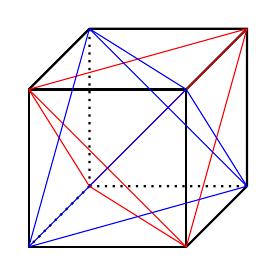
\begin{tikzpicture}[scale=2.0]
\draw[thick]
(0,0,1) -- (1,0,1) -- (1,1,1) -- (0,1,1) -- cycle;
\draw[thick]
(1,1,0) -- (1,1,1)
(1,0,0) -- (1,0,1)
(0,1,0) -- (0,1,1)
(1,0,0) -- (1,1,0) -- (0,1,0);
\draw[thick,dotted]
(0,0,0) -- (1,0,0)
(0,0,0) -- (0,1,0)
(0,0,0) -- (0,0,1);

\draw[red]
(1,0,1) -- (1,1,0) -- (0,1,1) -- cycle;
\draw[red]
(0,0,0) -- (1,0,1)
(0,0,0) -- (1,1,0)
(0,0,0) -- (0,1,1);

\draw[blue]
(1,1,1) -- (1,0,0)
(1,1,1) -- (0,1,0)
(1,1,1) -- (0,0,1);
\draw[blue]
(1,0,0) -- (0,1,0) -- (0,0,1) -- cycle;
\end{tikzpicture}

Beweise, dass $W$ auf der Menge dieser beiden Tetraeder operiert. Welche Symmetrien vertauschen die beiden Würfel, welche nicht?
\end{subproblem}

\begin{subproblem}
$W$ operiert auch auf der Menge der vier Raumdiagonalen

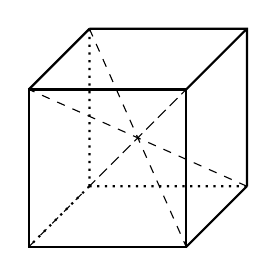
\begin{tikzpicture}[scale=2.0]
\draw[thick]
(0,0,1) -- (1,0,1) -- (1,1,1) -- (0,1,1) -- cycle;
\draw[thick]
(1,1,0) -- (1,1,1)
(1,0,0) -- (1,0,1)
(0,1,0) -- (0,1,1)
(1,0,0) -- (1,1,0) -- (0,1,0);
\draw[thick,dotted]
(0,0,0) -- (1,0,0)
(0,0,0) -- (0,1,0)
(0,0,0) -- (0,0,1);

\draw[dashed]
(0,0,0) -- (1,1,1)
(1,0,0) -- (0,1,1)
(0,1,0) -- (1,0,1)
(0,0,1) -- (1,1,0);
\end{tikzpicture}

Zeige, dass der dadurch definierte Homomorphismus $W\to Sym(4)$ surjektiv ist. Es gibt genau eine Symmetrie $s\in W$, die nicht die Identität ist, aber trotzdem auf das neutrale Element von $Sym(4)$ abgebildet wird. Welche?
\end{subproblem}
\begin{subproblem}
Die sechs Seitenmittelpunkte bilden die Ecken eines Oktaeders. Die acht Seitenmittelpunkte eines Oktaeders bilden einen Würfel.

\begin{tabular}{cc}
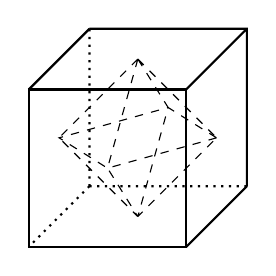
\begin{tikzpicture}
\draw[thick]
(-1,-1,+1) -- (+1,-1,+1) -- (+1,+1,+1) -- (-1,+1,+1) -- cycle;
\draw[thick]
(+1,+1,-1) -- (+1,+1,+1)
(+1,-1,-1) -- (+1,-1,+1)
(-1,+1,-1) -- (-1,+1,+1)
(+1,-1,-1) -- (+1,+1,-1) -- (-1,+1,-1);
\draw[thick,dotted]
(-1,-1,-1) -- (+1,-1,-1)
(-1,-1,-1) -- (-1,+1,-1)
(-1,-1,-1) -- (-1,-1,+1);

\draw[dashed]
(+1,0,0) -- (0,0,+1) -- (-1,0,0) -- (0,0,-1) -- cycle;
\draw[dashed]
(0,+1,0) -- (+1,0,0) -- (0,-1,0)
(0,+1,0) -- (0,0,+1) -- (0,-1,0)
(0,+1,0) -- (-1,0,0) -- (0,-1,0)
(0,+1,0) -- (0,0,-1) -- (0,-1,0);

\end{tikzpicture} &
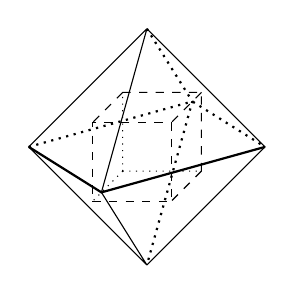
\begin{tikzpicture}[scale=0.5]
\draw[dashed]
(-1,-1,+1) -- (+1,-1,+1) -- (+1,+1,+1) -- (-1,+1,+1) -- cycle;
\draw[dashed]
(+1,+1,-1) -- (+1,+1,+1)
(+1,-1,-1) -- (+1,-1,+1)
(-1,+1,-1) -- (-1,+1,+1)
(+1,-1,-1) -- (+1,+1,-1) -- (-1,+1,-1);
\draw[dotted]
(-1,-1,-1) -- (+1,-1,-1)
(-1,-1,-1) -- (-1,+1,-1)
(-1,-1,-1) -- (-1,-1,+1);

\draw[thick]
(+3,0,0) -- (0,0,+3) -- (-3,0,0);
\draw[thick,dotted]
(-3,0,0) -- (0,0,-3) -- (+3,0,0);
\draw
(0,+3,0) -- (+3,0,0) -- (0,-3,0)
(0,+3,0) -- (0,0,+3) -- (0,-3,0)
(0,+3,0) -- (-3,0,0) -- (0,-3,0);
\draw[thick,dotted]
(0,+3,0) -- (0,0,-3) -- (0,-3,0);
\end{tikzpicture}
\end{tabular}

Daher operiert die Würfelgruppe auch als Symmetriegruppe eines Oktaeders, d.h. es gibt einen Homomorphismus $W\to O$. Umgekehrt gibt es einen Homomorphismus $O\to W$. Mache dir klar, dass es sich dabei um zwei zueinander inverse Abbildungen handelt. Die Würfelgruppe und die Oktaedergruppe sind also gleich.
\end{subproblem}

Es sei nun $T$ die Tetraeder-Gruppe, d.h. die Isometriegruppe des regelmäßigen Tetraeders. 
\begin{subproblem}
Zeige: $T$ operiert auf der Menge der vier Eckpunkte des Tetraeders und der dazugehörige (so wie in a. definierte) Gruppenhomomorphismus $T\to Sym(4)$ ist bijektiv.
\end{subproblem}
\begin{subproblem}
Die Kantenmittelpunkte der sechs Kanten eines regulären Tetraeders bilden einen Oktaeder.

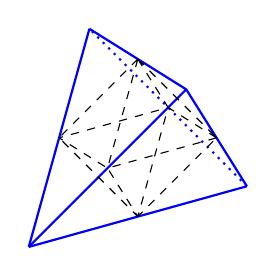
\begin{tikzpicture}
\draw[blue,thick]
(+1,+1,+1) -- (+1,-1,-1)
(+1,+1,+1) -- (-1,+1,-1)
(+1,+1,+1) -- (-1,-1,+1);
\draw[blue,thick,dotted]
(+1,-1,-1) -- (-1,+1,-1);
\draw[blue,thick]
(-1,+1,-1) -- (-1,-1,+1)
(-1,-1,+1) -- (+1,-1,-1);

\draw[dashed]
(+1,0,0) -- (0,0,+1) -- (-1,0,0) -- (0,0,-1) -- cycle;
\draw[dashed]
(0,+1,0) -- (+1,0,0) -- (0,-1,0)
(0,+1,0) -- (0,0,+1) -- (0,-1,0)
(0,+1,0) -- (-1,0,0) -- (0,-1,0)
(0,+1,0) -- (0,0,-1) -- (0,-1,0);
\end{tikzpicture}

Dies liefert uns einen Homomorphismus $T\to O$. Zeige, dass dieser injektiv, aber nicht surjektiv ist. Die Tetraeder ist also eine Untergruppe der Oktaedergruppe=Würfelgruppe, aber nicht gleich.
\end{subproblem}

\begin{subproblem}[difficulty={mittel bis schwer}]
Mache dir wie auch für die Würfel- und Oktaedergruppe klar, dass die Ikosaeder- und die Dodekaedergruppe gleich sind.

Finde außerdem einen nichttrivialen Homomorphismus $I\to Sym(5)$. (Hinweis: Im Dodekaeder gibt es fünf einbeschriebene Würfel).
\end{subproblem}
\end{problem}


\begin{problem}[title={Operation auf Teilmengen durch Konjugation}]
Sei $G$ eine Gruppe. Zeige: $G$ operiert auf der Potenzmenge $\Set{X | X\subseteq G}$ aller Teilmengen von $G$ durch Konjugation, d.h.
\[{^g X} := gXg^{-1} := \set{gxg^{-1} | x\in X}\]

Zeige außerdem:
\begin{subproblem}
$G$ operiert auch auf der Menge der Untergruppen von $G$.
\end{subproblem}
\begin{subproblem}
Wenn $G$ auf $\Omega$ operiert, dann sind Stabilisatoren von Punkten in derselben Bahn zueinander konjugiert. Konkret:
\[\forall g\in G, x\in\Omega: G_{^g x} = {^g G_x}\]
\end{subproblem}

Wieso interessiert uns das? Zeige:
\begin{subproblem}
Wenn $X,Y\subseteq\IR^n$ kongruente geometrische Objekte sind (z.B. zwei Würfel, zwei reguläre Tetraeder, ...), dann sind $\Aut(X)$ und $\Aut(Y)$ zueinander konjugierte, aber nicht unbedingt gleiche Untergruppen von $Isom(\IR^n)$.
\end{subproblem}
D.h. wenn wir die Symmetriegruppen von geometrischen Objekten bestimmen wollen, dann wollen wir eigentlich (bestimmte) Untergruppen von $Isom(\IR^n)$ \emph{bis auf Konjugation} bestimmen, denn natürlich wollen wir Untergruppen, die von kongruenten Objekten kommen, als gleich ansehen.
\end{problem}


\begin{problem}[title={Injektiv = trivialer Kern}]
Seien $G$ und $H$ Gruppen und $\phi:G\to H$ ein Gruppenhomomorphismus. Zeige
\[\phi\;\text{injektiv} \iff (\forall x\in G: \phi(x)=1 \implies x=1)\]
\end{problem}

\begin{problem}
Es seien $G,H,K$ Gruppen und $\phi: G\to H$, $\psi: H\to K$ Gruppenhomomorphismen zwischen ihnen. Zeige:

\begin{enumerate}
\item $\psi\circ\phi$ ist auch ein Gruppenhomomorphismus.
\item Ist $\phi$ bijektiv, so ist $\phi^{-1}:H\to G$ ebenfalls ein Gruppenhomomorphismus.
\end{enumerate}
\end{problem}

\begin{problem}
Sei $G$ eine Gruppe. Zeige, dass
\[\operatorname{Aut}(G) := \Set{\phi: G\to G | \phi\,\text{ist ein Gruppenisomorphismus}}\]
zusammen mit der Komposition eine Gruppe ist.

Es sei nun $\kappa_g: G\to G, x\mapsto gxg^{-1}$ der Konjugationsautomorphismus. Zeige, dass gilt:
\begin{enumerate}
\item $\kappa: G\to\operatorname{Aut}(G), g\mapsto\kappa_g$ ist ein Gruppenhomomorphismus ist.
\item Ist $\alpha: G\to G$ ein beliebiger Gruppenautomorphismus, so gilt $\alpha\circ\kappa_g\circ\alpha^{-1} = \kappa_{\alpha(g)}$.
\end{enumerate}
\end{problem}

\begin{problem}[title={Cayley-Einbettung; \enquote{Jede Gruppe ist eine Permutationsgruppe}}]
Sei $G$ eine Gruppe. Für jedes $g\in G$ sei $\lambda_g: G\to G, x\mapsto gx$ die Linksmultiplikationsabbildung.

Zeige, dass $\lambda: G\to Sym(G), g\mapsto\lambda_g$ ein injektiver Gruppenhomomorphismus ist.
\end{problem}

\begin{problem}
Zeige, dass
\[\operatorname{Aff}(\IR)\to\operatorname{GL}_2(\IR), aX+b \mapsto \begin{pmatrix} a & b \\ 0 & 1 \end{pmatrix}\]
ein Gruppenhomomorphismus ist. Ist er injektiv?
\end{problem}

\begin{problem}
Zeige, dass
\[\operatorname{GL}_2(\IC)\to \Set{\text{Möbius-Trafos}}, \begin{pmatrix} a & b \\ c & d \end{pmatrix} \mapsto \frac{aZ+b}{cZ+d}\]
ein Gruppenhomomorphismus ist. Ist er injektiv?
\end{problem}

\begin{problem}[title={Permutationsmatrizen}]
Zeige, dass $\phi: Sym(n) \to GL_n(\IR)$ mit
\[(\phi(\pi))_{ij} := \begin{cases} 1 & i=\pi(j) \\ 0 & \text{sonst} \end{cases}\]
ein Gruppenhomomorphismus ist. Vergewissere dich, dass für die Vektoren der Standardbasis $e_1,\ldots,e_n\in\IR^n$ gilt: $\phi(\pi)\cdot e_m = e_{\pi(m)}$, d.h. $\phi(\pi)$ permutiert die Elemente der Standardbasis genau so, wie $\pi$ die Elemente von $\set{1,\ldots,n}$ permutiert.
\end{problem}


\end{sheet}